\documentclass[11pt, oneside]{article}   	% use "amsart" instead of "article" for AMSLaTeX format
\usepackage{geometry}                		% See geometry.pdf to learn the layout options. There are lots.
\geometry{letterpaper}                   		% ... or a4paper or a5paper or ... 
%\geometry{landscape}                		% Activate for for rotated page geometry
%\usepackage[parfill]{parskip}    		% Activate to begin paragraphs with an empty line rather than an indent
\usepackage{graphicx}				% Use pdf, png, jpg, or eps� with pdflatex; use eps in DVI mode
								% TeX will automatically convert eps --> pdf in pdflatex		
\usepackage{amssymb}
\usepackage{amsmath}
\usepackage{parskip}
\usepackage{color}
\usepackage{hyperref}

\title{Solving the spring equation}
%\author{The Author}
%\section{}
%\subsection*{}
\date{}							% Activate to display a given date or no date

\graphicspath{{/Users/telliott_admin/Dropbox/Tex/png/}}
% \begin{center} 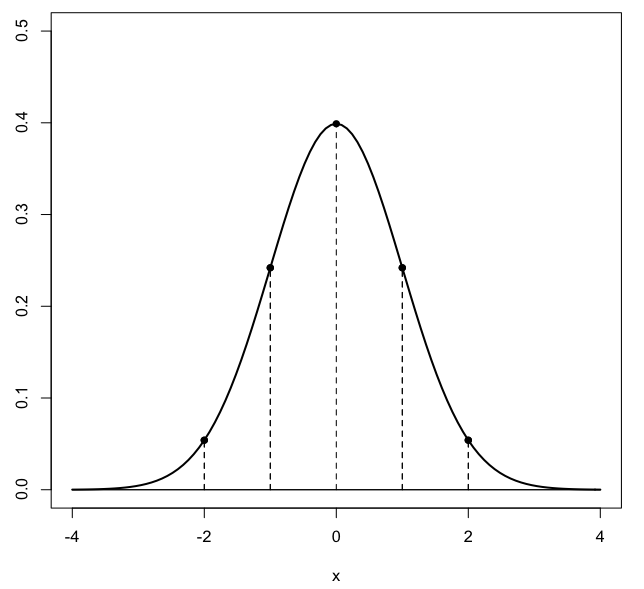
\includegraphics [scale=0.4] {gauss3.png} \end{center}
\begin{document}
\maketitle
\Large
The spring equation describes the motion of a mass attached to a spring on a frictionless table.  The mass is pulled to extend the spring, and then released.  The equation is
\[ F = ma = m \ddot x = -kx \]
Rearranging
\[ \ddot x + \frac{k}{m}x = 0 \]
One solution is
\[ x(t) = A \cos \omega t \]
\[ \ddot{x} = - \omega^2 A \cos \omega t \]
\[ (- \omega^2 + \frac{k}{m}) A \cos \omega t = 0 \]
since $A=0$ is a trivial solution, and $\cos \omega t$ cannot be always zero, we have
\[ \omega^2 = \frac{k}{m} \]
We can also try an exponential
\[ x(t) = A e^{\alpha t} \]
\[ \ddot{x} = \alpha^2 A e^{\alpha t} = \alpha^2 x \]
but this doesn't work, because $\alpha^2 \ge 0$, but $k$ and $m$ are both positive.
\subsection*{friction}
We can add a term in $\dot{x}$.
\[ \ddot{x} + b \dot{x} + cx = 0 \]
Now try the exponential
\[ x = A e^{\omega t} \]
\[ \dot{x} = \omega A e^{\omega t} \]
\[ \ddot{x} = \omega^2 A e^{\omega t} \]
so
\[ (\omega^2 + b \omega + c) A e^{\omega t} = 0 \]
becomes a quadratic 
\[ \omega^2 + b \omega + c = 0 \]
with solution
\[ \omega = -\frac{b}{2} \pm \sqrt{(\frac{b}{2})^2 - c} \]
Now there are various possibilities depending on the values of $b$ and $c$.  There are real solutions for $c \le b/2$.  For both $\pm$ the second term, $\omega$ is negative.  Then
\[ x(t) = Ae^{-|\omega|t} \]
dies out with time, which is what we expect to happen.  

There are also solutions for $c > b/2$.
\[ \omega = -\frac{b}{2} \pm i\sqrt{(c -\frac{b}{2})^2} \]
Define 
\[ \omega' = \sqrt{(c -\frac{b}{2})^2} \]
\[ \omega = -\frac{b}{2} \pm i \omega'  \]
\[ x(t) = A e^{-b/2} e^{\pm i \omega' t} \]
\subsection*{non-zero force}
\[ \ddot{x} + b \dot{x} + cx = d \]
The approach here is to say, rather than solve this equation, we will solve the equation for a complex number $z$ where
\[ \ddot{z} + b \dot{z} + cz = d \]
because the real part of $z$ will also be a solution, and using $z$ makes the manipulations easier.

We guess
\[ z = A e^{i \omega t} \]
\[ \dot{z} = i \omega A e^{i \omega t} \]
\[ \ddot{z} = - \omega^2 A e^{i \omega t} \]
We use the following trick.  $z$ containing both $\pm i$ are solutions, so add them together
\[ z = A e^{i \omega t} + B e^{-i \omega t}\]
Second, we need to take the real part of this.  The way that works is to add the complex conjugate of $z$, which requires that $B = A^*$ so
\[ x = \frac{1}{2} (A e^{i \omega t} + A^* e^{-i \omega t}) \]




\end{document}  